% Drawing 12/06-1 -- folder 12, batch 06, archive page 115 (PDF page 116).
% Transcription: en bas à droite, un diagramme des couples $(p, q)$ admissibles : deux axes, et des croix en escalier --- sur l'axe horizontal et les trois rangées au-dessus, trois croix à gauche puis, plus à droite, trois, trois, deux et une croix ; en haut de l'axe vertical, deux croix à la hauteur $n-1$ et une à la hauteur $n$. L'axe vertical est gradué « $1$ », « $2$ », …, « $n-1$ », « $n$ », l'axe horizontal, à droite, « $n-3$ », « $n-2$ », « $n-1$ ».
% Kind: lattice diagram of the admissible (p, q). Method 2 (schematic redraw from the facsimile). Status: ok.
% Notes: The two axes and the crosses as counted on the page, row by row from the horizontal axis upwards: 6 (three at the left, three at the right), 6, 5 (three and two), 4 (three and one); then, after a gap, 2 at height n-1 and 1 at height n on the vertical axis. Each cross is placed where he drew it (rows and columns are not regularised). Labels: 1, 2, n-1, n along the vertical axis; n-3, n-2, n-1 under the three right-hand columns. The gap between the left and the right columns, and between the lower rows and the two top rows, stands for the dots of « 1, 2, ..., n-1, n ». Redrawn 2026-11-12 (issue 128): to check again.
% Coordinates: 1 unit = 0.7 mm = 1/100 of the crop width (bbox in page fractions: [0.68, 0.71, 0.95, 0.835]).
% Redrawn by Claude (claude-fable-5-2), issue #128, 2026-11-12; not checked by a human; not compiled (no TeX in the session).
% Rights: reproduces part of the work -- behind RENDER_TRANSCRIPTS, never published by itself.
\documentclass[tikz,border=3pt]{standalone}
\usepackage{amsmath,amssymb}
\usetikzlibrary{patterns,arrows.meta}
\tikzset{pencil/.style={black!45}, struck/.style={black!35}, mpt/.style={circle,draw,inner sep=1.3pt}, pt/.style={circle,fill,inner sep=0.9pt}, opt/.style={circle,draw,fill=white,inner sep=1.1pt}}
\begin{document}
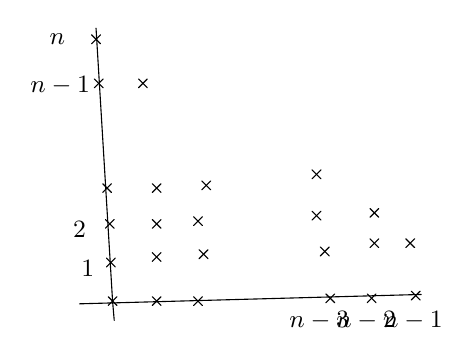
\begin{tikzpicture}[x=0.7mm,y=0.7mm,line cap=round,line join=round,font=\scriptsize]
\draw (21,-11) -- (24,-60.5) -- (24.3,-64);
\draw (18,-61) -- (80,-59.3);
\draw (23.2,-59.7) -- (24.8,-61.3);
\draw (23.2,-61.3) -- (24.8,-59.7);
\draw (31.2,-59.7) -- (32.8,-61.3);
\draw (31.2,-61.3) -- (32.8,-59.7);
\draw (38.7,-59.7) -- (40.3,-61.3);
\draw (38.7,-61.3) -- (40.3,-59.7);
\draw (62.7,-59.2) -- (64.3,-60.8);
\draw (62.7,-60.8) -- (64.3,-59.2);
\draw (70.2,-59.2) -- (71.8,-60.8);
\draw (70.2,-60.8) -- (71.8,-59.2);
\draw (78.2,-58.7) -- (79.8,-60.3);
\draw (78.2,-60.3) -- (79.8,-58.7);
\draw (22.9,-52.7) -- (24.5,-54.3);
\draw (22.9,-54.3) -- (24.5,-52.7);
\draw (31.2,-51.7) -- (32.8,-53.3);
\draw (31.2,-53.3) -- (32.8,-51.7);
\draw (39.7,-51.2) -- (41.3,-52.8);
\draw (39.7,-52.8) -- (41.3,-51.2);
\draw (61.7,-50.7) -- (63.3,-52.3);
\draw (61.7,-52.3) -- (63.3,-50.7);
\draw (70.7,-49.2) -- (72.3,-50.8);
\draw (70.7,-50.8) -- (72.3,-49.2);
\draw (77.2,-49.2) -- (78.8,-50.8);
\draw (77.2,-50.8) -- (78.8,-49.2);
\draw (22.7,-45.7) -- (24.3,-47.3);
\draw (22.7,-47.3) -- (24.3,-45.7);
\draw (31.2,-45.7) -- (32.8,-47.3);
\draw (31.2,-47.3) -- (32.8,-45.7);
\draw (38.7,-45.2) -- (40.3,-46.8);
\draw (38.7,-46.8) -- (40.3,-45.2);
\draw (60.2,-44.2) -- (61.8,-45.8);
\draw (60.2,-45.8) -- (61.8,-44.2);
\draw (70.7,-43.7) -- (72.3,-45.3);
\draw (70.7,-45.3) -- (72.3,-43.7);
\draw (22.2,-39.2) -- (23.8,-40.8);
\draw (22.2,-40.8) -- (23.8,-39.2);
\draw (31.2,-39.2) -- (32.8,-40.8);
\draw (31.2,-40.8) -- (32.8,-39.2);
\draw (40.2,-38.7) -- (41.8,-40.3);
\draw (40.2,-40.3) -- (41.8,-38.7);
\draw (60.2,-36.7) -- (61.8,-38.3);
\draw (60.2,-38.3) -- (61.8,-36.7);
\draw (20.7,-20.2) -- (22.3,-21.8);
\draw (20.7,-21.8) -- (22.3,-20.2);
\draw (28.7,-20.2) -- (30.3,-21.8);
\draw (28.7,-21.8) -- (30.3,-20.2);
\draw (20.2,-12.2) -- (21.8,-13.8);
\draw (20.2,-13.8) -- (21.8,-12.2);
\node[inner sep=1pt] at (14,-13) {\small $n$};
\node[inner sep=1pt] at (14.5,-21.5) {\small $n-1$};
\node[inner sep=1pt] at (18,-47.5) {\small $2$};
\node[inner sep=1pt] at (19.5,-54.5) {\small $1$};
\node[inner sep=1pt] at (61.5,-64) {\small $n-3$};
\node[inner sep=1pt] at (70,-64) {\small $n-2$};
\node[inner sep=1pt] at (78.5,-64) {\small $n-1$};
\end{tikzpicture}
\end{document}
